\capitulo{3}{Conceptos teóricos}


Esta sección auna los diferentes conocimientos teóricos necesarios para la realización del proyecto. A continuación, y en este orden, se explicarán los algoritmos utilizados, protocolos de comunicación y sistemas físicos empleados.

\section{Algoritmia}


\subsection{Filtros de Partículas}

Los Filtros de Partículas son modelos utilizados para tratar de estimar el estado de un sistema que cambia con el tiempo. 
\\Fue definido como \textit{bootstrap filter} en 1993 por N. Gordon, D. Salmond y A. Smith.  Se trata de un método que pretende implementar filtros bayesianos recursivos, haciendo uso del método de Montecarlo, es decir, realiza repetidas medidas del estado para estimar la posición del sistema.
\\ 

\subsection{Campos Potenciales}

A la hora de lograr una navegación segura en un entorno determinado, es necesario implementar un sistema de evasión de obstáculos. 
\\Introducido por Oussama Khatib en 1986, el algoritmo de Campos Potenciales aporta una manera de evitar colisionar con los diferentes obstáculos existentes.\\ Se basa en la idea de que el agente se mueve en un campo de fuerzas. La posición que debe alcanzar, su meta o destino, se presenta como una fuerza de atracción, y los obstáculos como fuerzas repulsivas. 
Los diferentes vectores fuerza, determinan la dirección y magnitud de la fuerza atrayente o repulsora.\\Sea $q$ la posición actual del agente, considerada como una partícula moviendose en un espacio n-dimensional $R^n$. Por simplicidad, se considera la posición como una tupla, esto es, bidimensional, tal que $q = (x,y)$. El campo potencial en el que se encuentra el agente se una función escalar $ U(q):R^2\rightarrow R $, generado por la superposición de los campos atrayentes $U_{att}$ y repulsores $U_{rep}$:
$$U(q) = U_{att}(q) + U_{rep}(q)$$

Por supuesto, la suma de todos lo campos repulsores $U_{rep}$ generan un vector repulsor, que sumado al de atracción puede determinar la necesidad de acercarse o alejarse de una determinada zona:
$$U(q) = U_{att}(q) + \sum_i{U_{rep_i}(q)}$$

Donde $U_{rep_i}$ representa el campo potencial generado por un obstáculo $i$.

Suponiendo que $U(q)$ es diferenciable, en cada punto $q$, el campo potencial $\nabla(q)$ es un vector que apunta en la dirección que, \textbf{localmente}, incrementa $U(q)$. \\De esta forma, si el potencial de atracción en la meta se considera 0 y a medida que el agente se distancia de ella, se incrementa, se puede establecer, teniendo en cuenta el potencial de repulsión producido por los diferentes obstáculos, un vector $F(q)$ cuya dirección apunta hacia donde se reduce el potencial $U$, y su magnitud establece la velocidad con que este se reduce:
$$ F(q) = F_{att}(q) + F_{rep}(q) = -\nabla U_{att}(q) - \nabla U_{rep}(q) $$



\textbf{El potencial de atracción} $U_{att}(q)$ se establece como una función cuadrática proporcional a la distancia a la meta. De esta forma crece exponencialmente a medida que el agente se aleja de su destino, y se reduce considerablemente en su cercanía. Así puede ser utilizado como fuente de información para establecer la velocidad de aproximación al objetivo, de forma que el agente no sobreactue:
$$U_{att}(q) = \epsilon * \delta_{meta}(q)^2$$
Donde $\delta$ es la distancia euclidiana desde la posición del agente $q$ a la meta $meta$, y $\epsilon$ es un factor de escalado positivo, que puede utilizarse para ajustar la influencia de la distancia en la velocidad del agente. Y su gradiente negativo: 
$$ -\nabla U_{att}(q) = -\epsilon * (q - q_{meta}) $$

\begin{figure}[H]
	\centering
	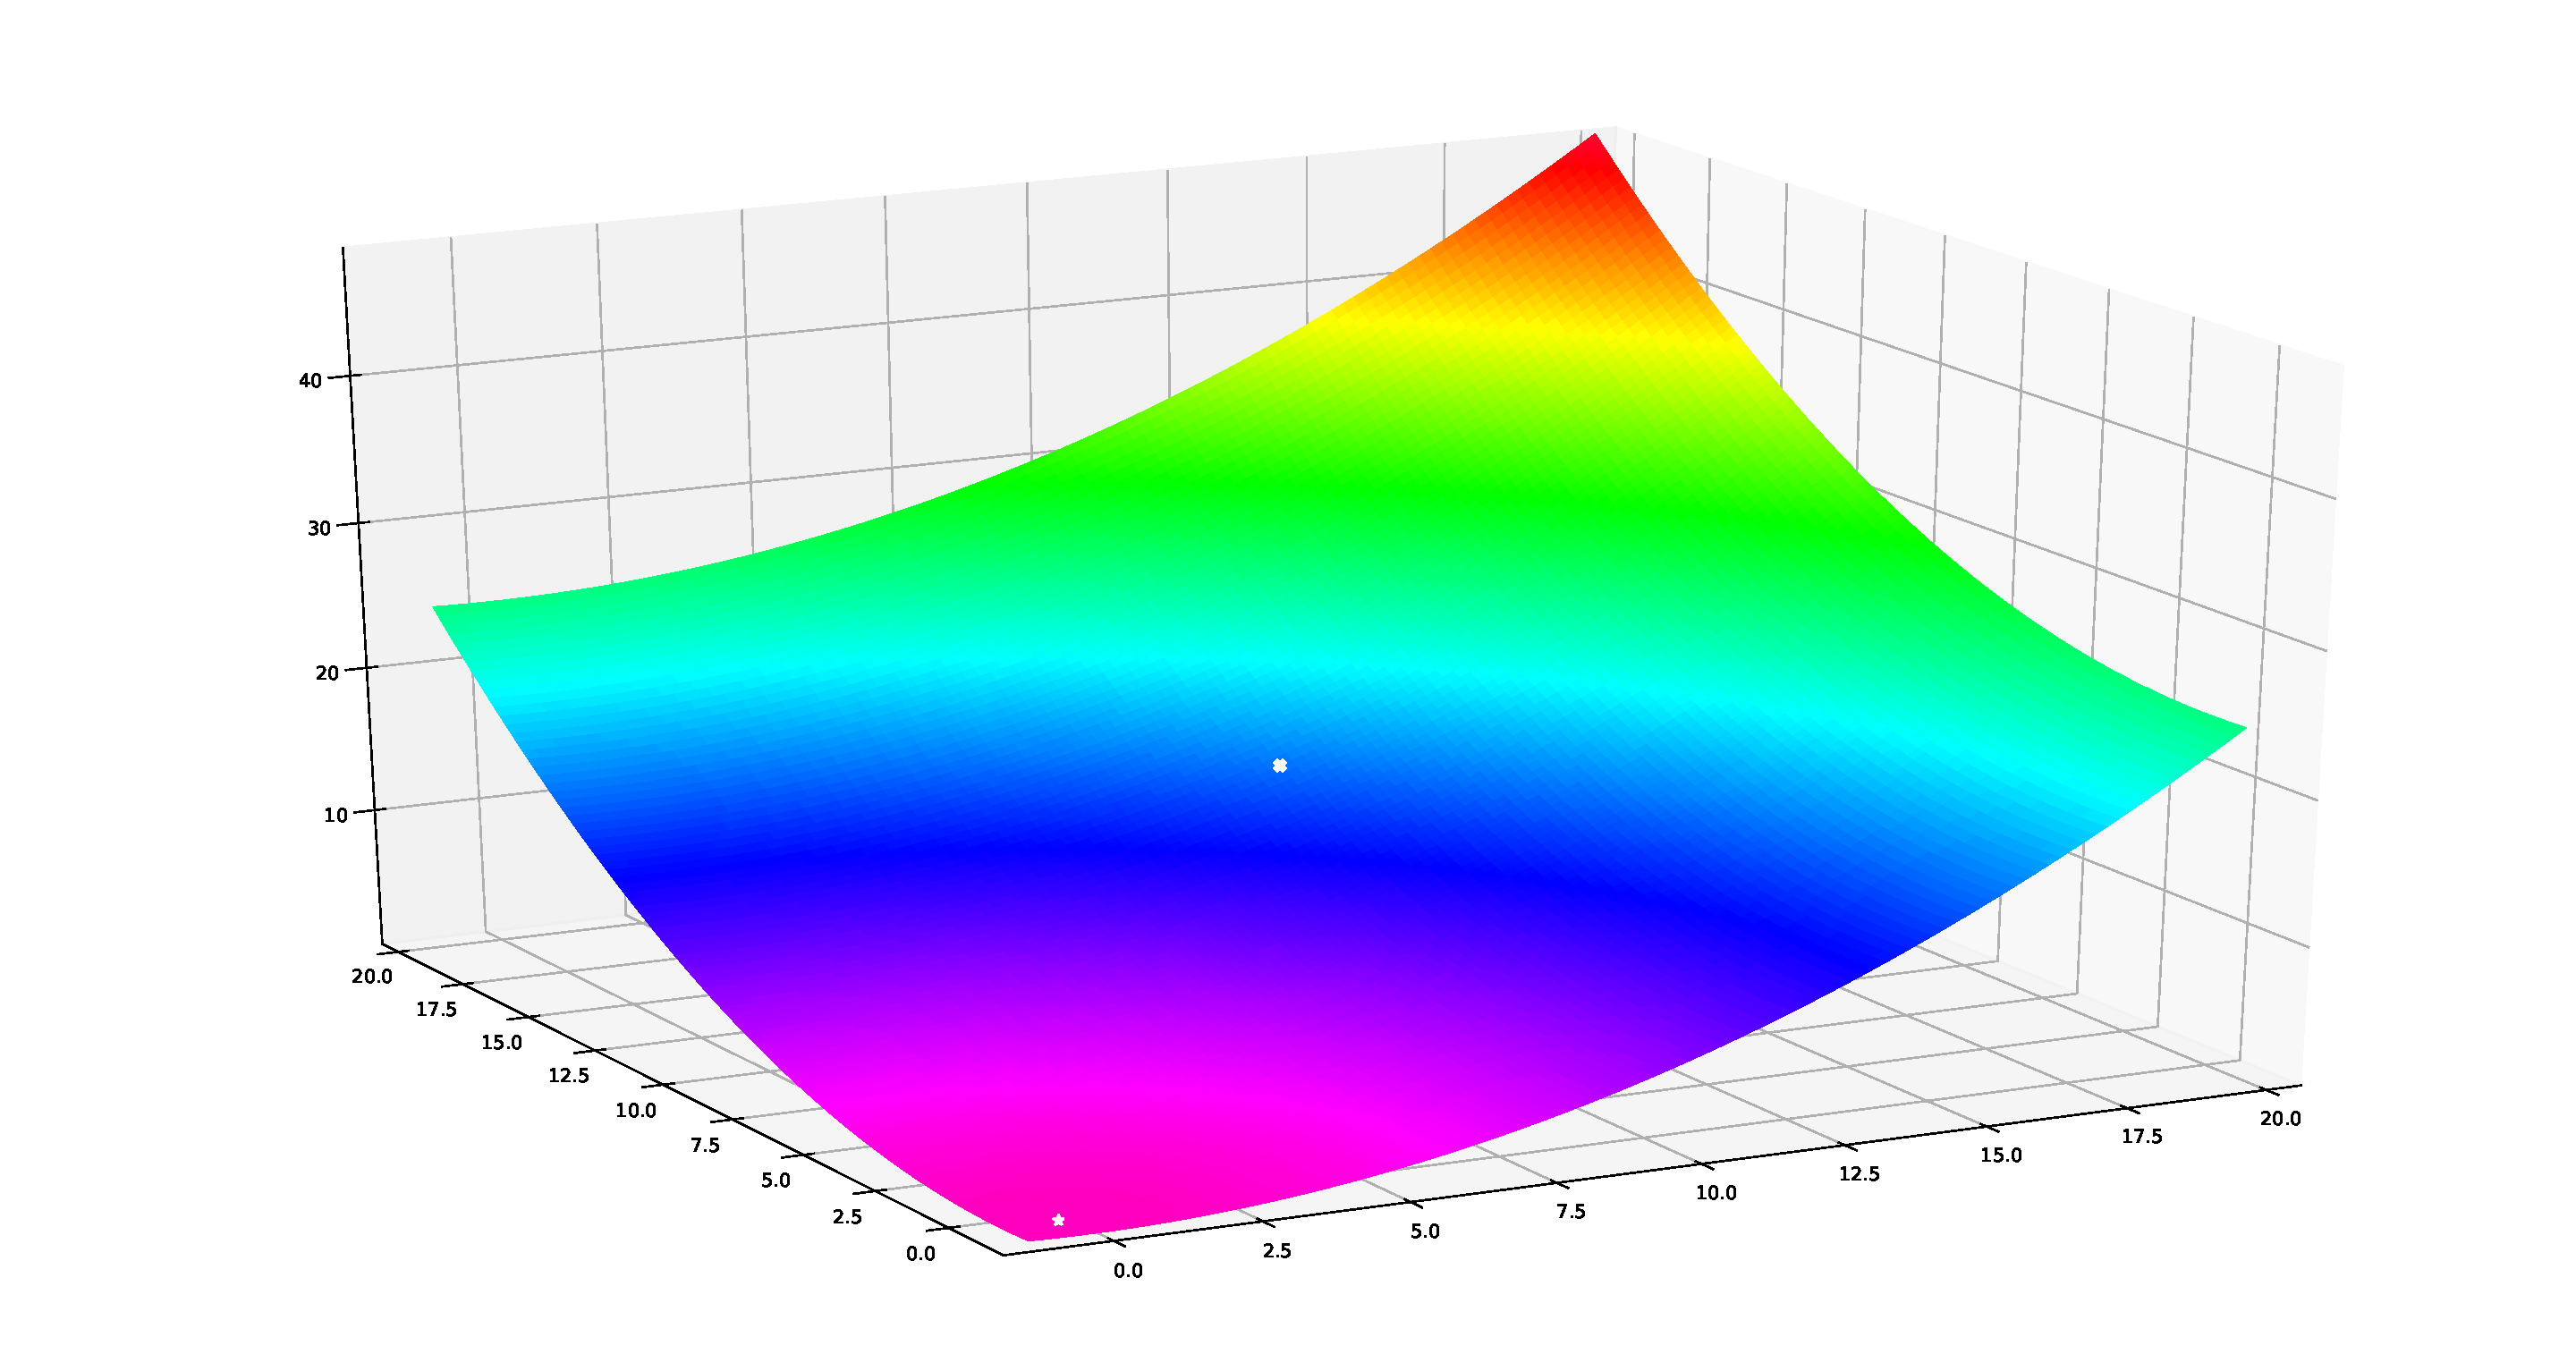
\includegraphics[width=\textwidth]{UattrGradient}
	\caption{Gradiente de Potencial de Atracción.}\label{fig:uattrgrad}
\end{figure}

En la figura \ref{fig:uattrgrad} se ha establecido el agente en el punto $(10,12)$ y la meta en $(0,0)$. Puede verse el efecto del gradiente aplicado.

\textbf{El potencial de repulsión} $U_{rep}(q)$ lo establecen los obstáculos detectados por los sensores del agente. Si se establece una función proporcional a la distancia del agente a los obstáculos, el potencial repulsor crece en la cercanía a estos, y decrece con la distancia. De esta forma un obstáculo lejano al agente no debería presentar niguna fuerza sobre él:
$$U_{rep}(q) = U = \begin{cases}
0 & \text{ si } \delta > \rho \\ 
\eta * (\frac{1}{\delta_{obs}(q)}-\frac{1}{\rho})^2 & \text{ si } \delta \leq \rho; \delta \neq 0 
\end{cases}$$

Donde $\eta$ es un factor de escalado positivo, que permite establecer como de fuerte se ve afectado el agente por el campo repulsor, $\delta$ es la distancia euclidiana desde la posición del agente $q$ al obstáculo $obs$, y $\rho$ es un factor de escalado positivo, que permite establecer la distancia de influencia de forma proporcional. Y su gradiente
$$-\nabla U_{rep}(q) = \begin{cases} 0 & \text{ si } \delta > \rho \\
\eta * (\frac{1}{\delta_{obs}(q)}-\frac{1}{\rho}) * \frac{1}{\delta_{obs}(q)^2}\frac{q-q_{obs}}{\delta_{obs}(q)} & \text{ si }  \delta \leq \rho; \delta \neq 0  
\end{cases}$$

\begin{figure}[H]
	\centering
	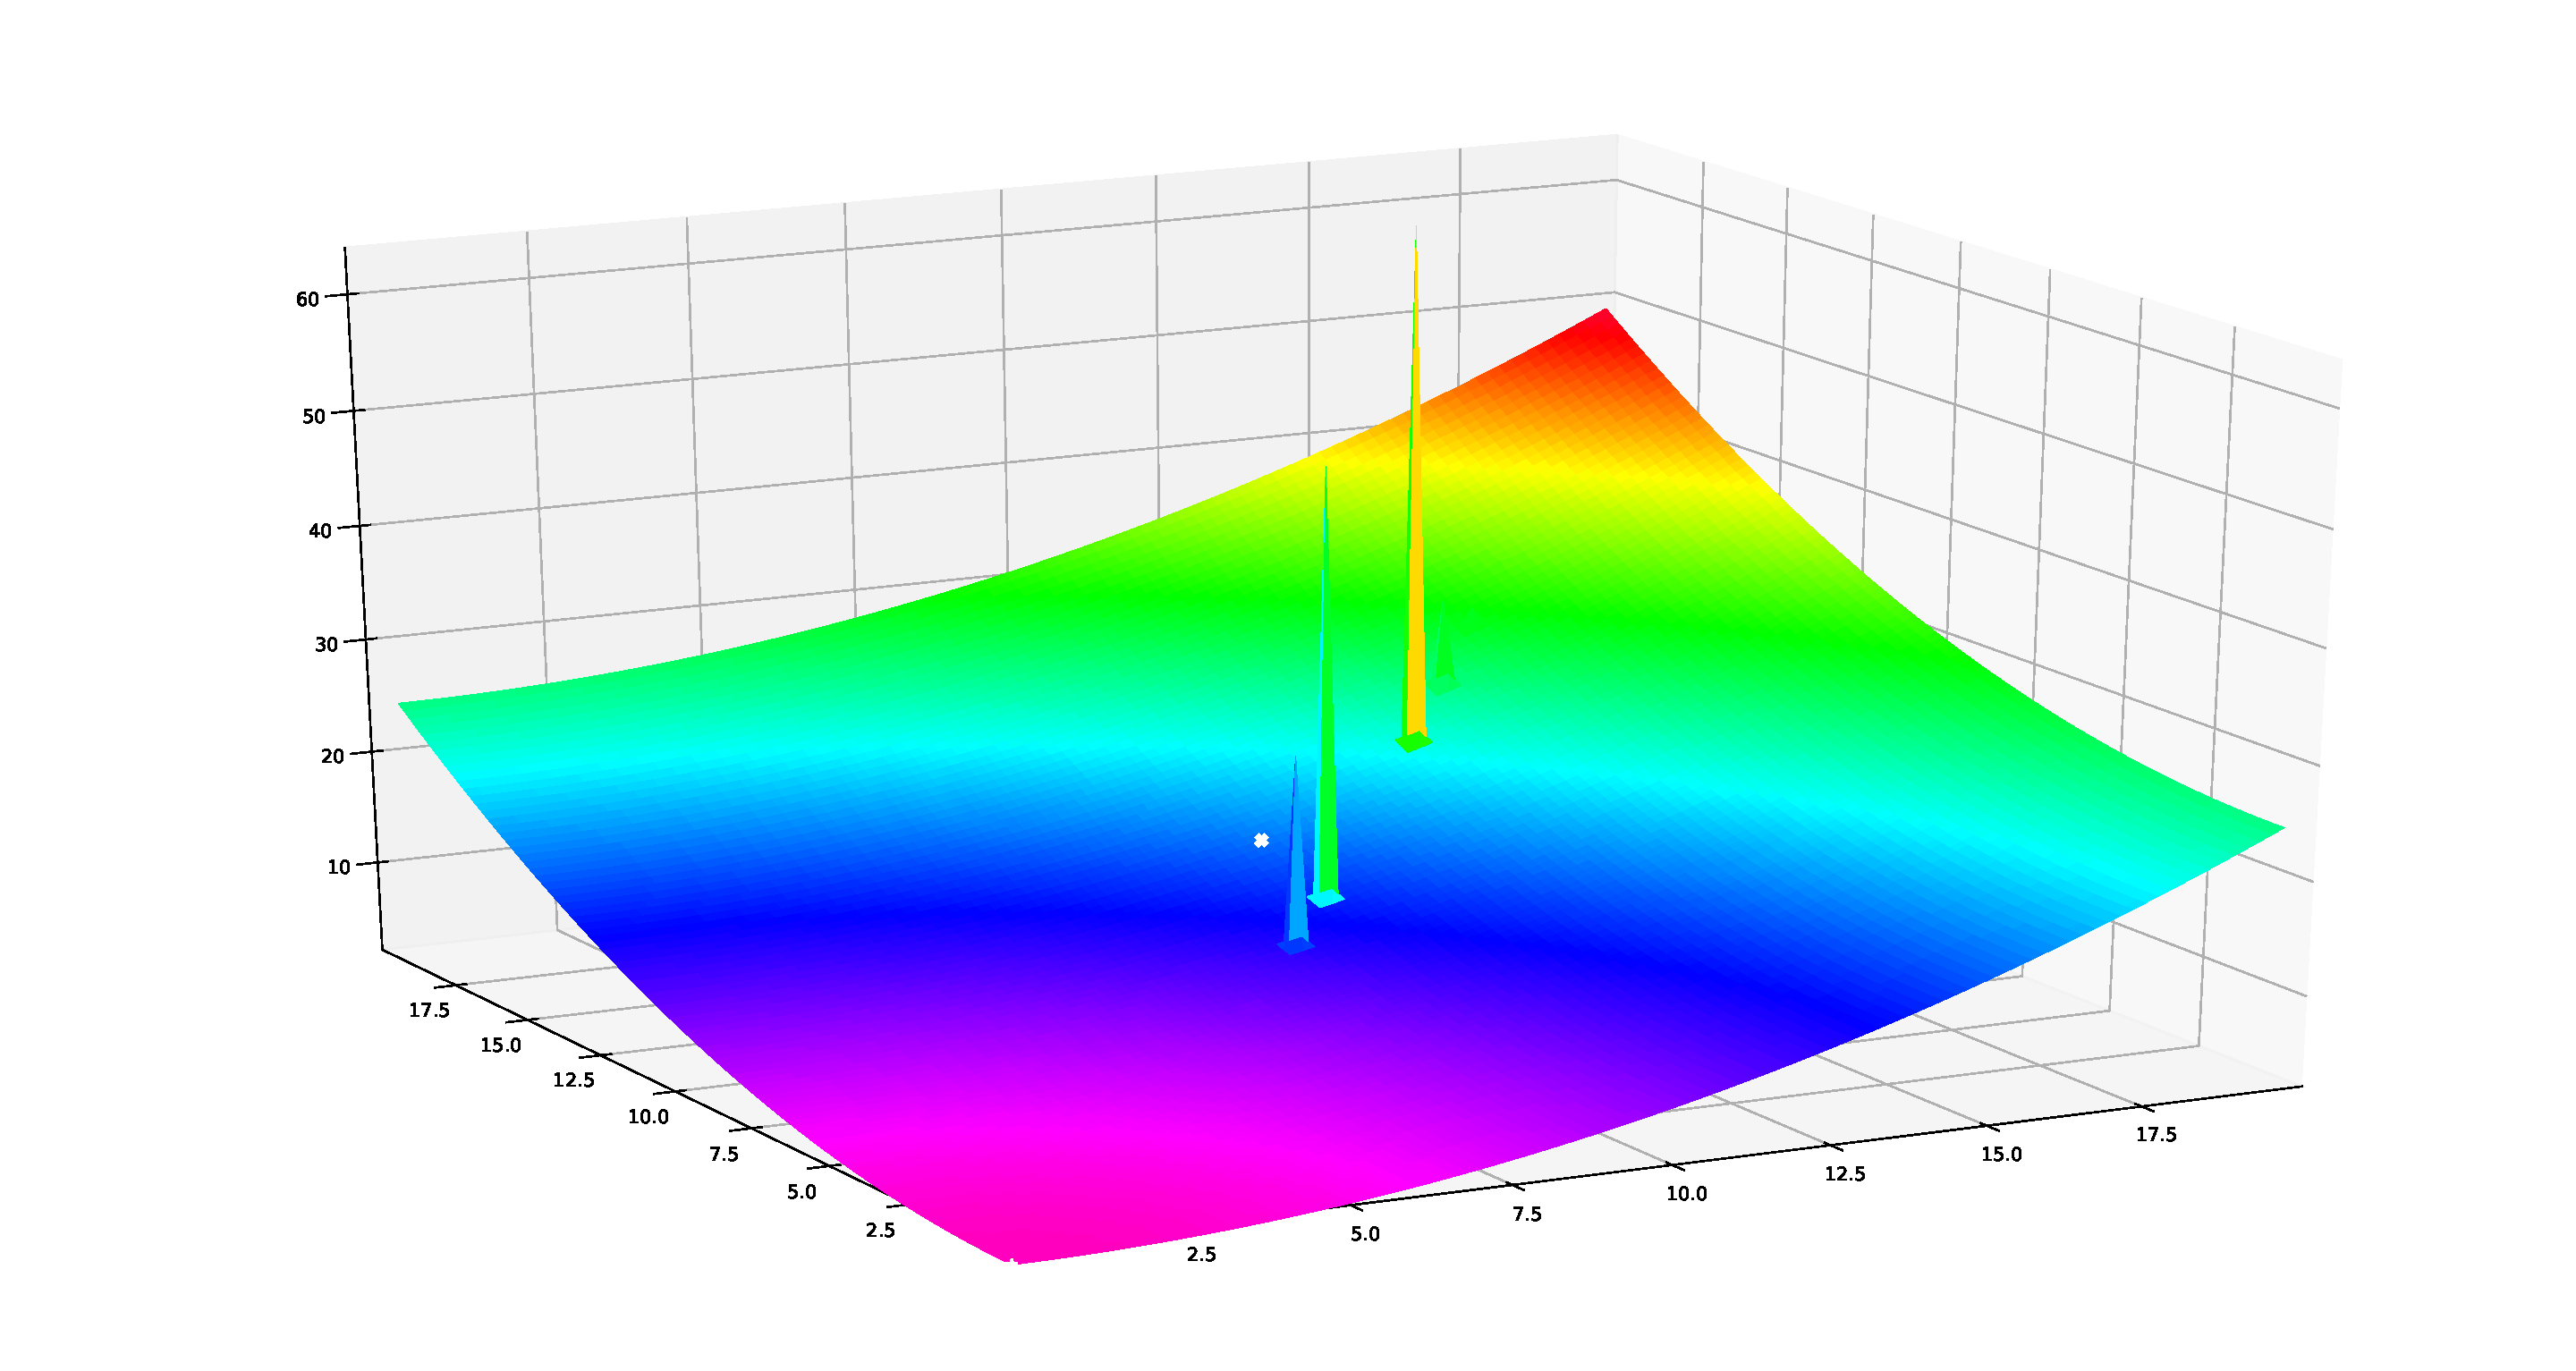
\includegraphics[width=\textwidth]{UrepGradient}
	\caption{Gradiente de Potencial de Repulsión.}\label{fig:urepgrad}
\end{figure}

 En la figura \ref{fig:urepgrad} se ha creado una serie de obstáculos artificialmente para ilustrar el comportamiento del algoritmo. 

 \newpage
\subsubsection{Desventajas}
El algoritmo de campos potenciales se puede llevar a cabo con una implemntación simple y eficiente haciendo uso de Numpy, dado que se puede crear una representación matricial del plano en que se desplaza el agente, que contenga los diferentes potenciales en cada posición. 
Esto hace sencillo realizar cálculo vectorizado sobre las matrices. \\Sin embargo, tiene ciertas desventajas que lo han hecho, cuanto menos, inútil para las necesidades de este proyecto:
\begin{itemize}
\item Es un algoritmo basado en descenso de gradiente, y como tal puede quedar \textit{atascado} en mínimos locales. Estos mínimos pueden encontrarse en zonas que contengan obstáculos en forma cóncava o de caja abierta, tal como se ilustra en la figura \ref{fig:localmin}.
\begin{figure}[H]
	\centering
	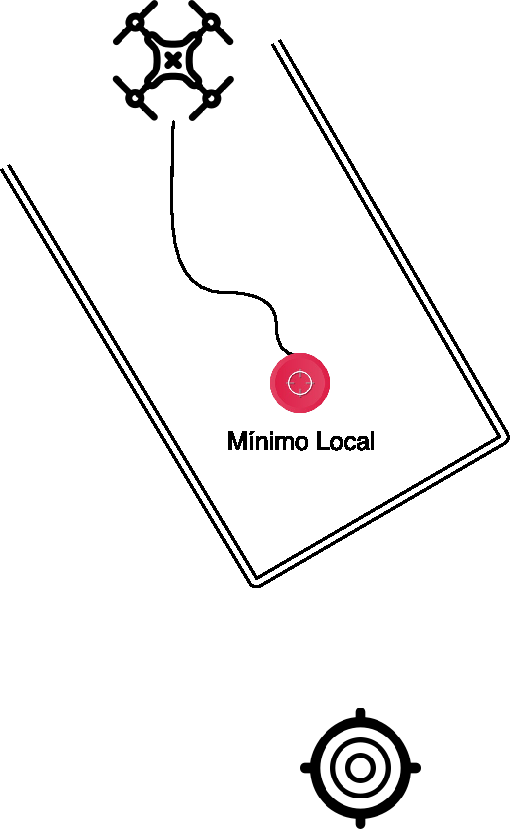
\includegraphics[width=0.5\textwidth]{localmin}
	\caption{Mínimo local en zonas convexas.}\label{fig:localmin}
\end{figure}
\item De encontrarse en un espacio con forma de corredor o pasillo, cualquier acercamiento hacia las paredes ocasionará una corrección en el sentido opuesto al campo repulsor, lo cual puede ocasionar un movimiento oscilatorio si dicha corrección supone aproximar el agente a la pared opuesta, tal y como se ilustra en la figura \ref{fig:corridoroverc}.
\begin{figure}[H]
	\centering
	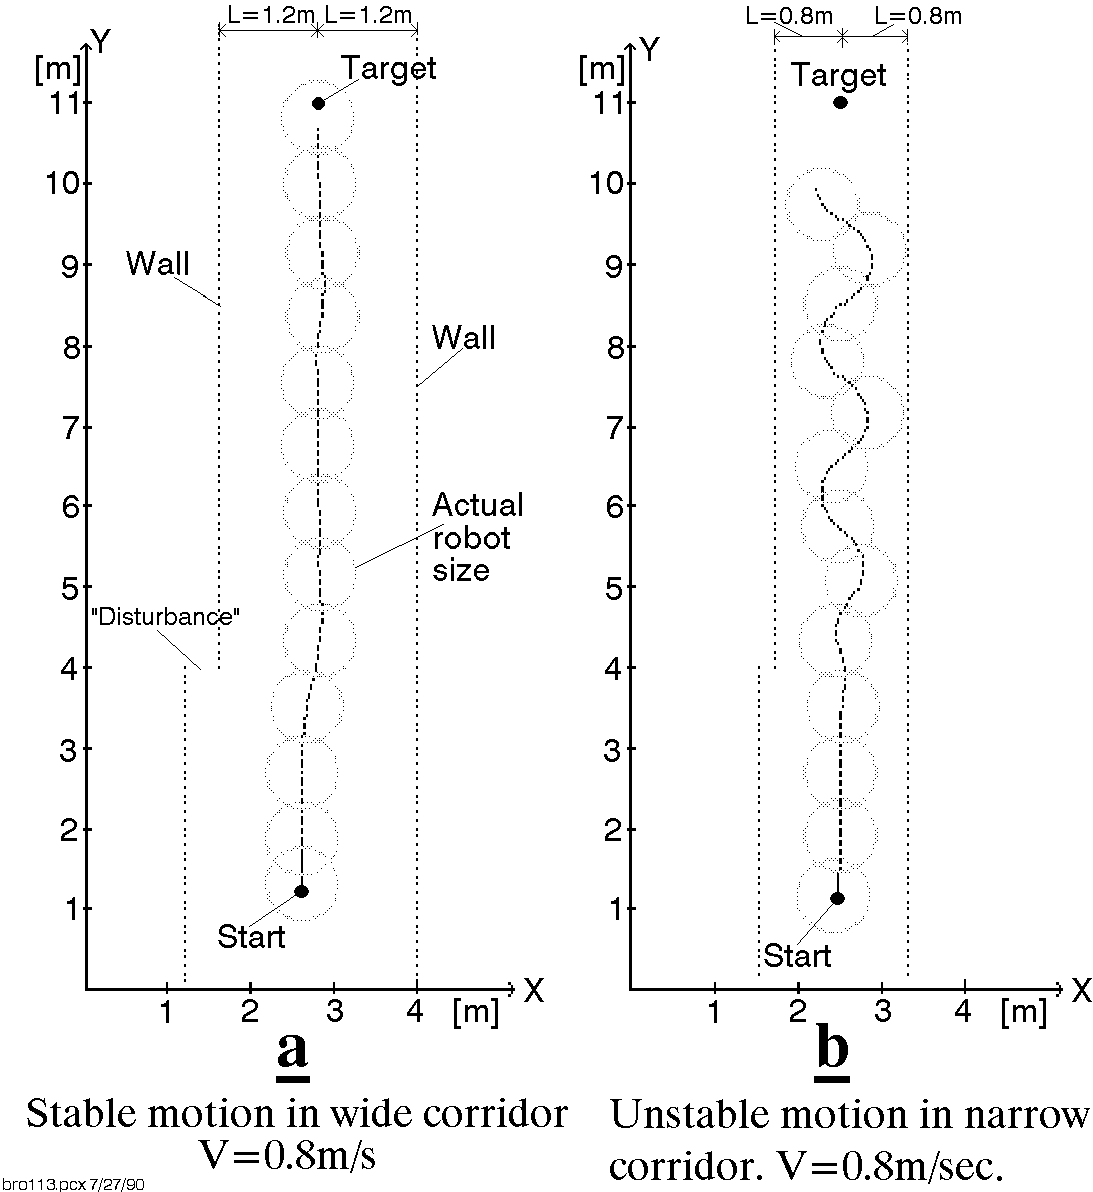
\includegraphics[width=0.5\textwidth]{corridoroverc}
	\caption{Movimiento oscilatorio en corredores estrechos.}\label{fig:corridoroverc}
\end{figure}
\item Alta complejidad computacional pese a poder modelarse como calculo vectorizado, requiere de muchas más operaciones que otros métodos más avanzados.
\item No funciona correctamente con agentes que se desplazan a alta velocidad. 
\item Al realizar la adición de todos los campos potenciales, tanto repulsores como atrayente, se produce una gran pérdida de información sobre la distribución local de los obstáculos.
\end{itemize} 

Por estos motivos, se ha desechado el algoritmo de Campos Potenciales como sistema de evasión de obstáculos, y se ha pasado a un modelo más avanzado basado en un plano cartesiano, conocido como \textit{Vector Field Histogram} y detallado en el apartado \nameref{subsec:VFH}. 
 
\subsection{Vector Field Histogram}
\label{subsec:VFH}
El Vector Field Histogram, o Histograma de Campos Vectoriales, \textit{VFH} de aquí en adelante, fue introducido por Borenstein y Korem en el año 1991. Permite la detección de obstáculos y su evasión mediante el control de la dirección y velocidad del agente en tiempo real.


\section{Dispositivos Físicos}

\subsection{Raspberry Pi}


\begin{table}[H]
	\begin{center}
		\rowcolors {2}{gray!35}{}
		\begin{tabular}{l | c}\hline
			\toprule
			Componente & Raspberry Pi 3B\\
			\otoprule
			CPU & BCM2837\\
			Núcleos & 4\\
			Velocidad & 1.2GHz\\
			RAM & 1GB\\
			Coms & Ethernet, WiFi, Bluetooth\\
			USB & 4 (2.0)\\
			GPIO & 40\\
			Consumo máximo & 6.7W\\
			\bottomrule
		\end{tabular}
		\caption{Componentes de una Raspberry Pi 3 Model B}
		\label{tb:raspi3hardware}
	\end{center}
\end{table}

\noindent Una Raspberry Pi es un pequeño ordenador desarrollado en UK por la Raspberry Pi Foundation, con la intención de promover el aprendizaje de informática básica en colegios y países en desarrollo. El modelo base se compone de una única placa de medidas 85mm x 56mm (LxA), y unos 42g de peso.\\Concretamente el modelo empleado es una Raspberry Pi 3B, y consta de los componentes detallados en la tabla \ref{tb:raspi3hardware}



\noindent Su reducido tamaño y bajo consumo lo hacen ideal para este tipo de proyecto. \\En este caso se utiliza bajo una distribución GNU/Linux llamada Raspbian\footnote{Descargable desde: https://www.raspberrypi.org/downloads/raspbian}, basada en Debian. Para tratar de mejorar su rendimiento y reducir al mínimo el consumo, se ha escogido la versión Lite del sistema, es decir, un sistema mínimo sin entorno de escritorio y con la mayor parte de servicios desactivados por defecto.

\begin{figure}
	\centering
	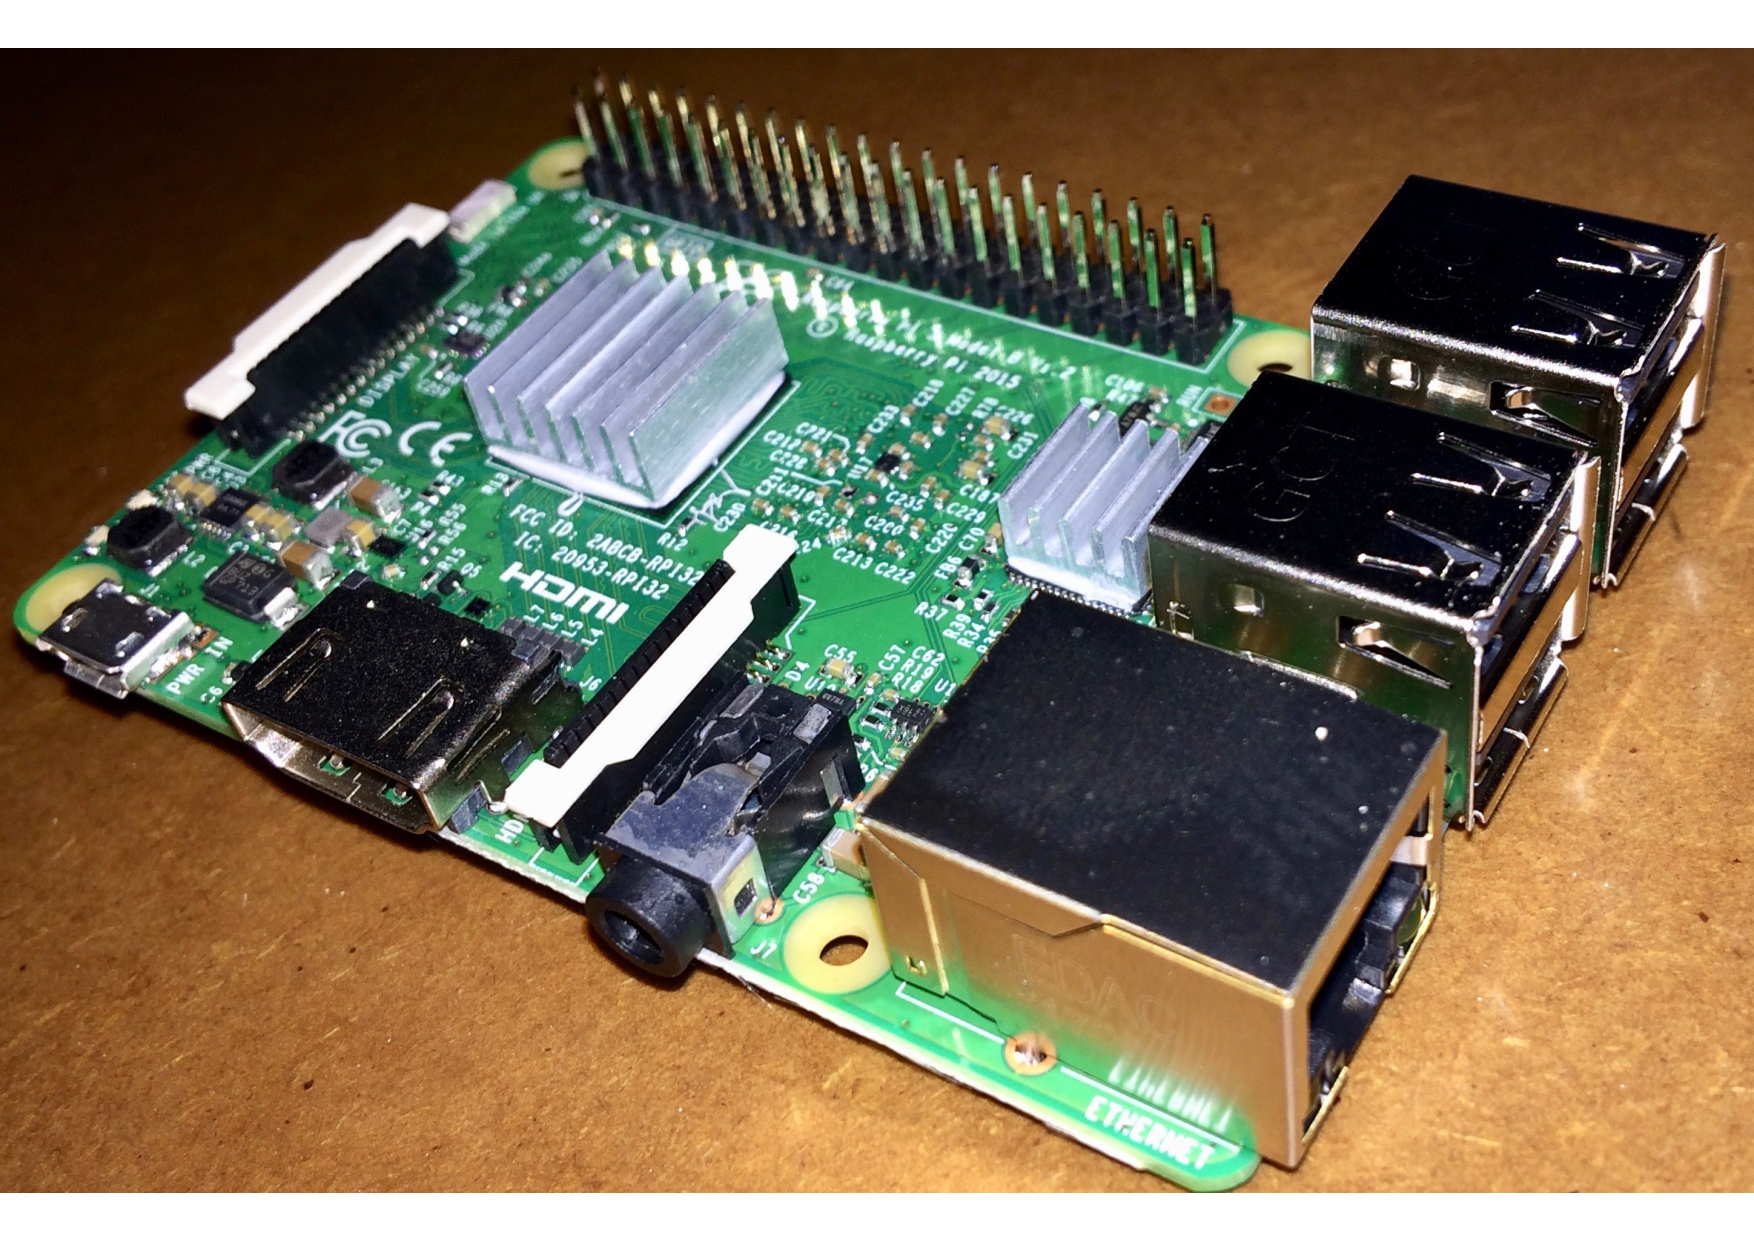
\includegraphics[width=0.9\textwidth]{raspi}
	\caption{Raspberry Pi 3.}\label{fig:raspi3b}
\end{figure}

Una vez descargado el sistema, este ha sido instalado en una micro SD mediante el siguiente procedimiento por consola\footnote{Realizado en OSX, aunque en Linux es muy similar}:
\begin{itemize}
\item\code{diskutil list} Permite localizar el dispositivo en el que se encuentra la tarjeta. En nuestro caso \code{/dev/disk4}
\item\code{diskutil umountDisk /dev/disk4} Permite desmontar el volumen. 
\item\code{sudo dd if=raspbian-stretch.img of=/dev/rdisk4 bs=1m} El comando \code{dd} copia la entrada estándar a la salida estándar. Mediante \code{if/of} se establece el fichero de entrada/salida. Mediante \code{bs} se establece el tamaño de bloque a copiar. Se está utilizando \code{/dev/\underline{\textbf{r}}disk4} en lugar de \code{/dev/disk4} debido a la capacidad de OSX de trabajar con dispositivos en bruto, \textit{raw}, de forma que es posible acceder al dispositivo de forma directa\footnote{Véase \code{man hdiutil}, sección \textit{DEVICE SPECIAL FILES}}, sin almacenar en un buffer la lectura del archivo, proporcionando velocidades de escritura/lectura hasta 20 veces más rápidas.
\end{itemize}


Una vez realizados estos pasos, se puede insertar la microSD en la Raspberry Pi. Para encenderla basta con utilizar el puerto micro-usb de que dispone.\\La Raspberry Pi 3 requiere de una fuente de alimentación capaz de proporcionar 2,5A\footnote{Véase https://www.raspberrypi.org/help/faqs/\#power} para funcionar al máximo nivel de estrés para el procesador y alimentar dispositivos USB.

Sin embargo, este no es estrictamente nuestro caso, véase el apartado \hyperref[subsec:Modificaciones]{Modificaciones}. Se requiere un dispositivo cuyo consumo sea lo más reducido posible, pero que sea rápido en la ejecución, y que muestre poca latencia en operaciones de \code{IO}, que es donde se encuentra el cuello de botella.

Una vez encendida, se accede a ella con el usuario por defecto \code{pi} y la contraseña por defecto \code{raspberry}. Obviamente ambas \textbf{han sido cambiadas} por motivos de seguridad.



\subsubsection{Modificaciones}
\label{subsec:Modificaciones}

\begin{figure}
	\centering
	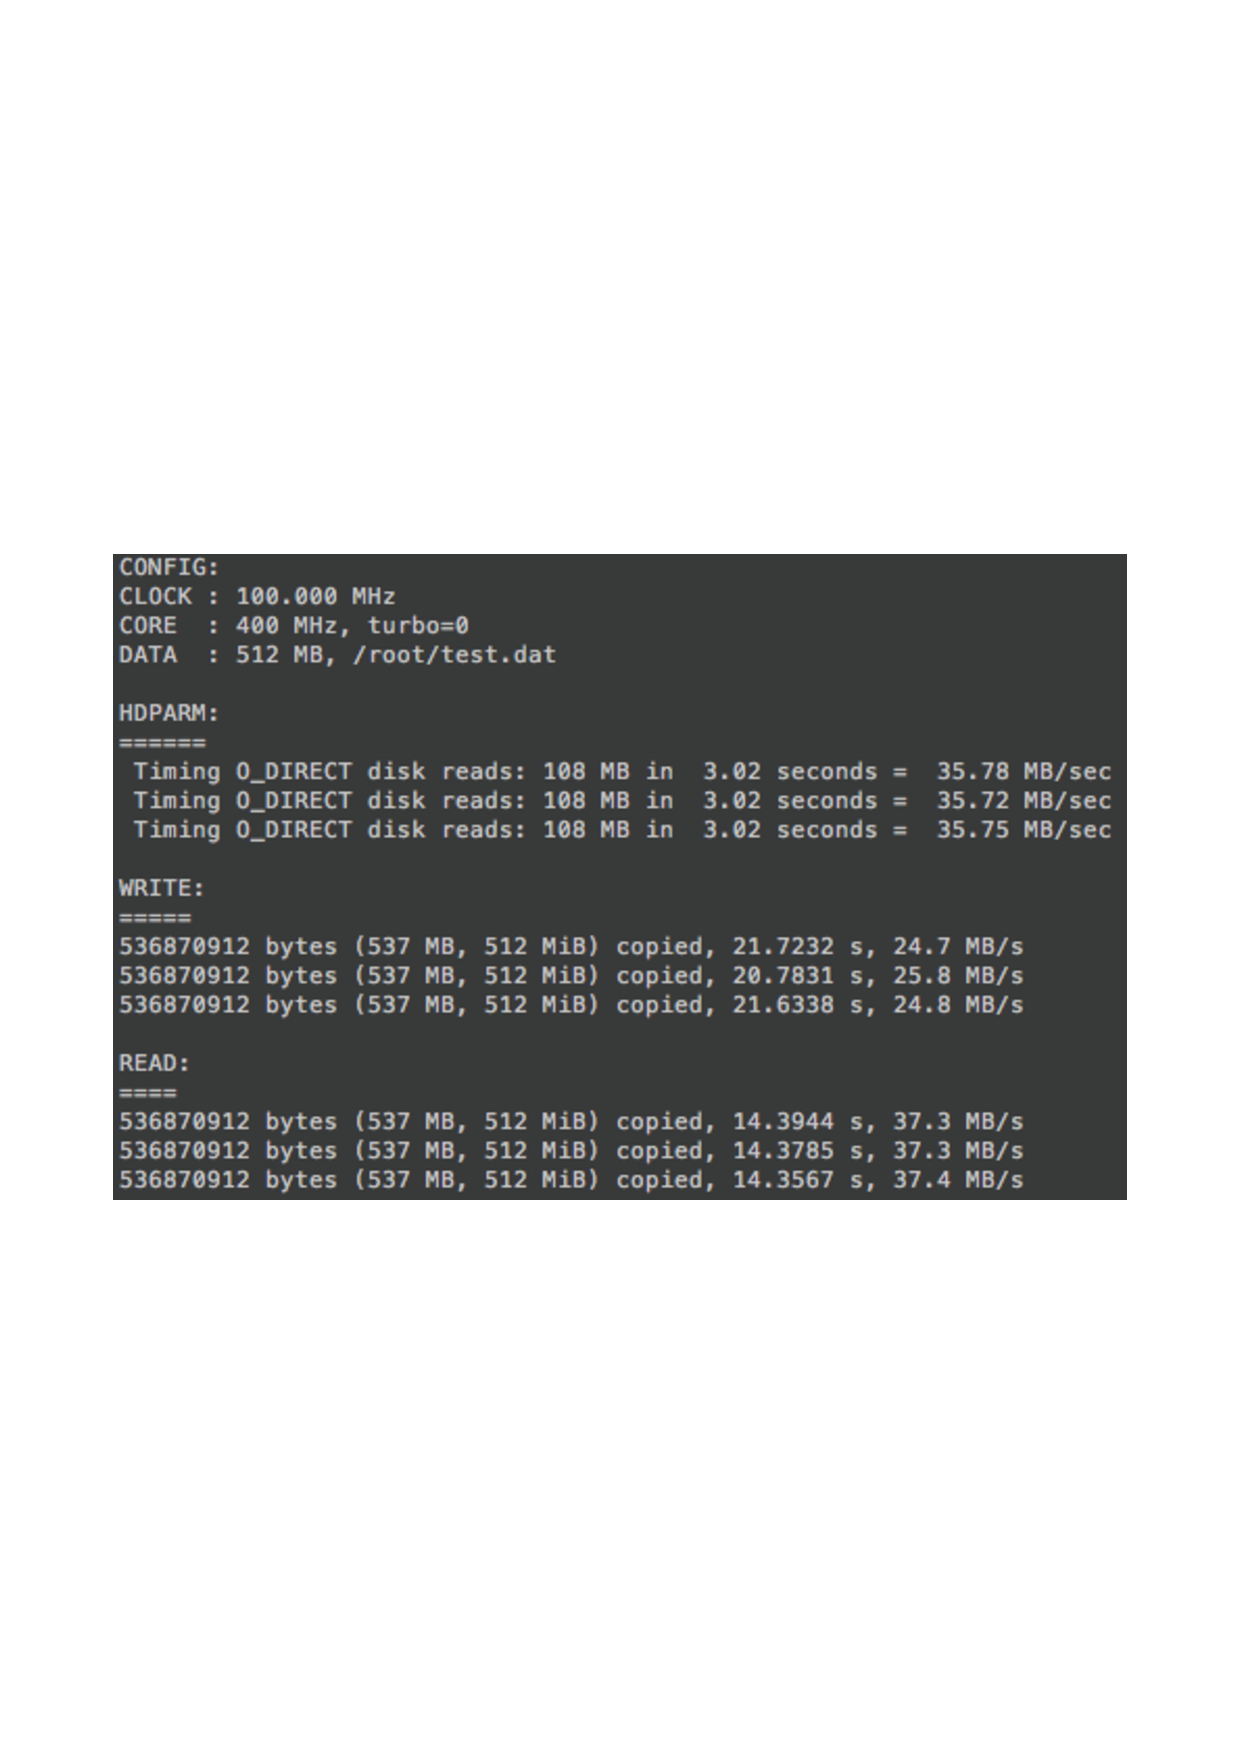
\includegraphics[width=0.9\textwidth]{sdbench}
	\caption{Benchmark de lector microSD OC.}\label{fig:sdbenchmark}
\end{figure}

\begin{itemize}
\item Se ha desactivado el puerto HDMI para reducir el consumo en \textasciitilde{}30mA: \\Para ello se ha incluido en \code{/etc/rc.local} la línea \code{/usr/bin/tvservice -o}.
\item Se ha overclockeado el lector de microSD a 100MHz, en lugar de los 50MHz por defecto: \\Para ello se ha incluido en \code{/boot/config.txt} la línea \code{dtparam=sd\_overclock=100}.\\Y que arroja los resultados mostrados en la imagen \ref{fig:sdbenchmark}
\item Se han incluido una serie de disipadores para evitar sobrecalentamiento de la placa. Así como un pequeño ventilador de bajo consumo.
\end{itemize} 


\subsection{Controladora de Vuelo}

Una controladora de vuelo (\textit{FC} de aquí en adelante) es un pequeño circuito integrado, que contiene un procesador, una serie de sensores, y una serie de entradas y salidas. 
\begin{figure}
\centering
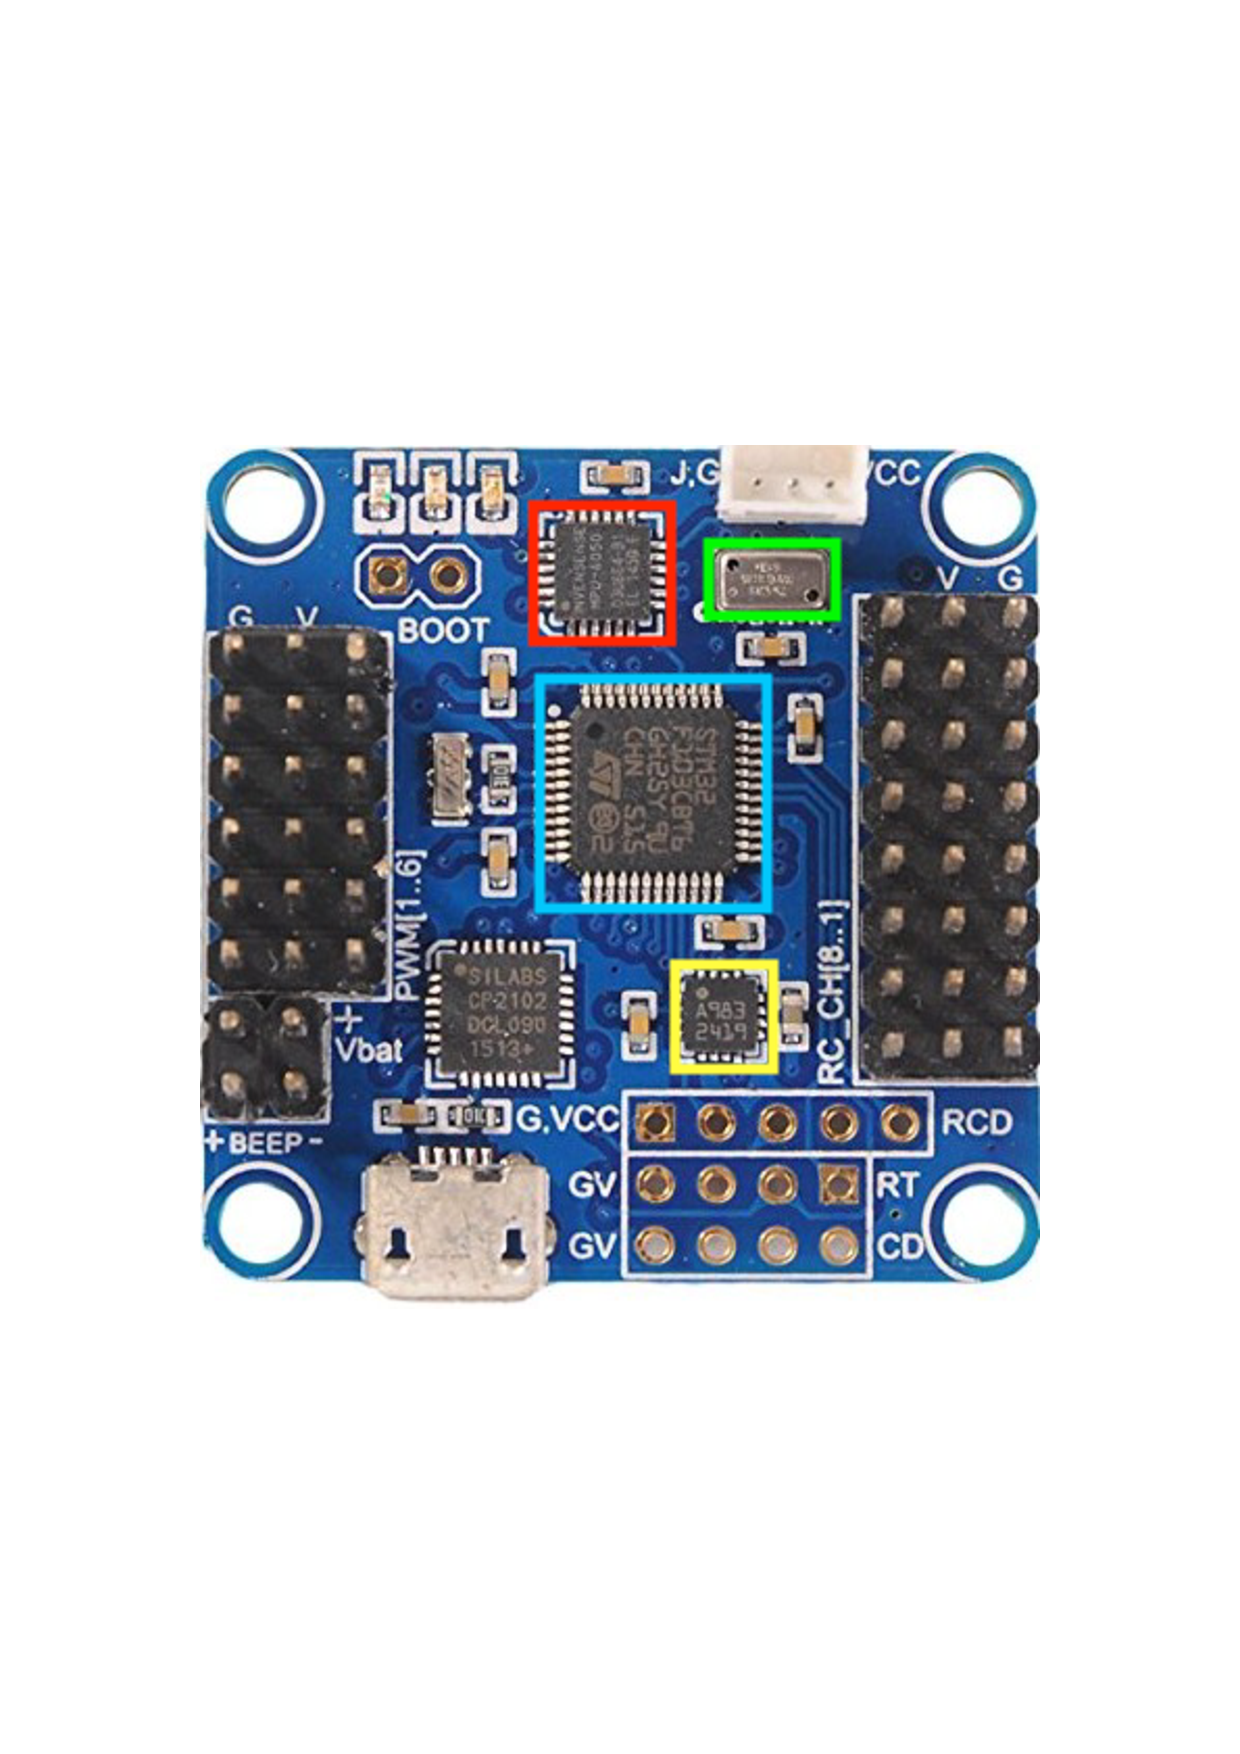
\includegraphics[width=0.5\textwidth]{flip32}
\caption{Controladora de Vuelo Flip32.}\label{fig:fc}
\end{figure}
La FC se encarga de mantener el sistema de estabilización del drone, tomando medidas de los sensores de que dispone, tales como un acelerómetro, giroscopio, magnetómetro, barómetro... etc. 

En el caso de la FC usada para este proyecto, llamada Flip32 y mostrada en la imagen \ref{fig:fc}, se dispone de un IC MPU-6050, en rojo, con acelerómetro y giroscopio, así como de un barómetro M55611, en verde, y un magnetómetro HMC5883L, en amarillo.
El núcleo de esta pequeña placa es un procesador STM32F103, en cyan, a 72MHz y basado en arquitectura ARM el cual dispone de dos puertos serie, que permiten establecer comunicación entre la FC y otros dispositivos, como emisoras u otros sensores.

El puerto micro-USB de que dispone es utilizado para establecer comunicación entre el configurador de opciones del drone, o en el caso de nuestro proyecto, para hacer uso del \hyperref[subsec:MSP]{MultiWii Serial Protocol}. 


\subsubsection{Entradas}
En el lado derecho de la imagen \ref{fig:fc} pueden verse una serie de pines que actúan como 8 canales de entrada desde el receptor de radio.
Dichos canales de entrada, por defecto, reciben una señal modulada en ancho de pulso o \hyperref[subsec:PWM]{PWM}

 

\subsubsection{Salidas}
En el lado izquierdo de la imagen \ref{fig:fc}, pueden verse otros pines que actúan como salida de señal hacia los controladores de velocidad de los motores del drone (ESC o \textit{Electronic Speed Controller}).
Estos pines de salida, emiten una señal que será interpretada por los ESC del drone, para determinar la frecuencia dada al voltaje que alimenta los motores. En el caso de nuestro proyecto, los ESC disponibles reciben una señal PWM, al igual que la FC desde un receptor de radio.

\newpage
\subsubsection{Sensores}
La controladora de vuelo Flip32 en su versión más completa, dispone de los siguientes sensores:
\begin{itemize}
\item IMU\footnote{Unidad de Medición Inercial.} MPU-6050: Se trata de un circuito integrado compuesto de un acelerómetro de tres (3) ejes y un giroscopio de tres (3) ejes. El acelerómetro mide las fuerzas en los tres diferentes ejes (en \textit{g}) , el giroscopio se encarga de medir la velocidad angular en cada uno de los tres ejes (en degº/s )
\item Magnetómetro HMC5883L: Se trata de un pequeño magnetómetro digital capaz de medir el campo magnético terrestre (en Gauss). Se debe tener en cuenta que según la posición en el planeta, el campo magnético varía entre \si{\gauss{0.25}} - \si{\gauss{0.65}}, así como la declinación magnética de la zona en la que se realiza la medición.\footnote{Disponible en: http://magnetic-declination.com/}
\item Barómetro M55611: Se trata de un altímetro de alta precisión, con resoluciones de hasta 10cm, que funciona midiendo la presión atmosférica (en milibar). Hay que tener en cuenta que los cambios de presión, como los generados por las hélices del drone, hacen variar la medida del sensor. Por ello, en el caso de usarlo, se cubre con un pequeño filtro de un material absorbente, lo suficientemente denso como para evitar el contacto directo entre una corriente de aire y el sensor.
\end{itemize}
\newpage
\section{Protocolos}

\subsection{Pulse Width Modulation}
\label{subsec:PWM}

\externaldocument[5-]{./tex/5_Aspectos_relevantes_del_desarrollo_del_proyecto}

La modulación por ancho de pulso, se basa en medir el transcurso de tiempo entre el flanco de subida de una señal, y el flanco de bajada, tal y como puede verse en la imágen \ref{fig:PWM}.
En este contexto, un receptor de radio recibe una señal de la emisora,  y genera una señal PWM acorde que será transmitida a la FC.
Estas son capaces de entender señales de entre 1000 y 2000\si{\us}. Cualquier valor por debajo, o por encima, haría entrar la controladora en FailSafe\footnote{Al recibir una señal inválida por parte del receptor, la controladora de vuelo puede ser configurada para desactivar el drone, mantener la última medida buena conocida, intentar aterrizar... etc. Este modo es conocido como FailSafe}
En el caso de este proyecto, se ha determinado que no se hará uso de este protocolo para la comunicación entre la Raspberry Pi y la controladora de vuelo, véase \ref{5-sec:MSP_implementation} y \ref{subsec:MSP}, y por lo tanto el uso de estos pines queda descartado.

Sin embargo, la comunicación entre la FC y los ESC se realiza mediante este tipo de señal, por ello se ha considerado relevante explicar, brevemente, su funcionamiento.
\begin{figure}
	\centering
	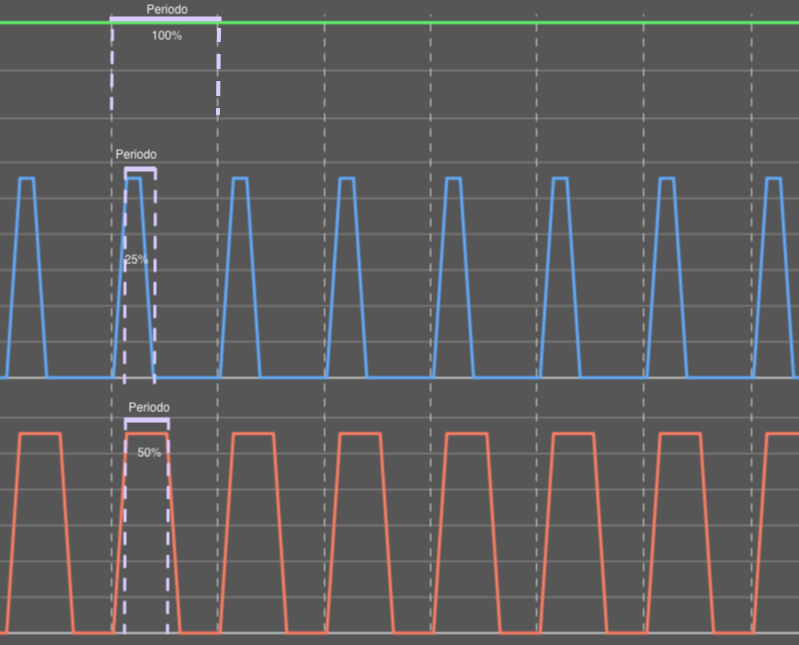
\includegraphics[width=0.9\textwidth]{PWM}
	\caption{Modulación en Ancho de Pulso. Arriba 100\% del ciclo usado. Centro 25\% del ciclo usado. Abajo 50\% del ciclo usado}\label{fig:PWM}
\end{figure}


\subsection{MultiWii Serial Protocol}
\label{subsec:MSP}

MultiWii es un software de control de multirotores y está basado en componentes de la Nintendo Wii. Concretamente, los mandos de control de la consola de Nintendo poseen tres acelerómetros para determinar la posición angular y medir aceleraciones laterales. El problema es que los acelerómetros no son precisos para variaciones pequeñas, de forma que Nintendo creó un complemento que se podía conectar al propio mando, el Wii Motion Plus, que dispone de tres giroscopios, de forma que unidos a los tres acelerómetros iniciales, proporcionan una medición mucho más precisa de la posición del mando.

A los primeros creadores del sistema de control MultiWii se les ocurrió la posiblidad de hacer uso de estos sensores para crear un sistema de control de drones. Uniendo estos sensores a un controlador, en principio se trató de un Arduino Mini, y programándolo para tal efecto, se logra crear una FC algo rudimentaria, pero que da muy buenos resultados.

Para crear un entorno amigable para el usuario común, se desarrolló una aplicación de escritorio capaz de configurar los parámetros de esta controladora de vuelo poco convencional. De alguna forma debía lograrse una comunicación entre la FC y la aplicación, y así se implementó MultiWii Serial Protocol.\\Conocido como \textit{MSP}, se trata de un protocolo que se ha mantenido en diferentes implementaciones de sistemas de control de vuelo. No solo aquellos basados en sensores de la Nintendo Wii controlados por Arduino, sino en otros más modernos y potentes que han ido surgiendo los últimos años. Como el utilizado en nuestro proyecto.

Es un protocolo eficiente y sencillo, que permite una comunicación rápida y completa. Su composición puede verse en la imagen \ref{fig:MSPlayout}
\begin{figure}
	\centering
	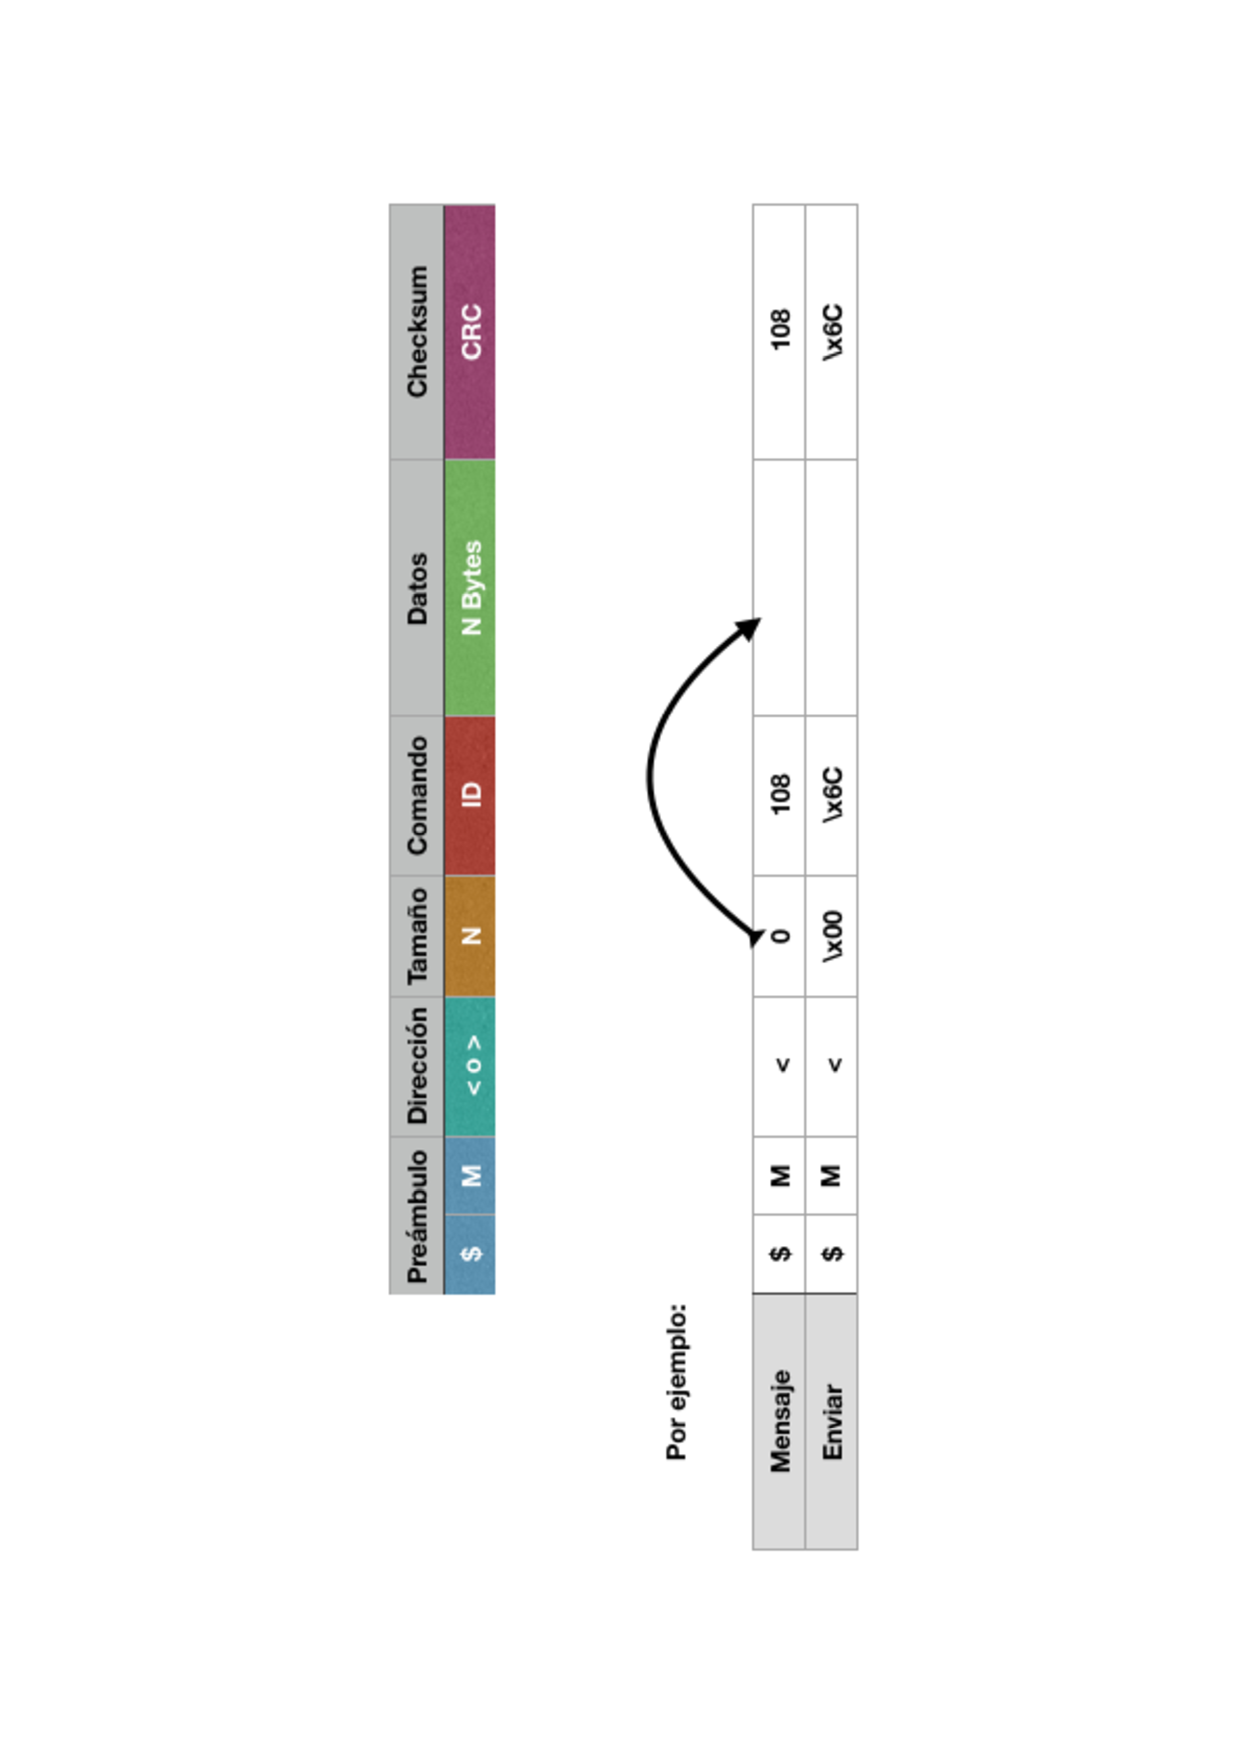
\includegraphics[width=0.9\textwidth]{MSPlayout}
	\caption{Composición de un mensaje MSP}\label{fig:MSPlayout}
\end{figure}

\begin{itemize}
\item Preámbulo: Se trata de dos caracteres ASCII que determinan el comienzo de un nuevo mensaje. Se compone de un símbolo '\$' y una letra 'M'.
\item Dirección: Se trata de un caracter ASCII que determina la dirección del mensaje, \textbf{hacia} la controladora '<' o \textbf{desde} la controladora '>'.
\item Tamaño: Se trata de un byte que determina el tamaño, en bytes, de los datos enviados o recibidos.
\item Comando: Se trata de un byte que determina el comando a ejecutar. Véase \ref{5-sec:MSP_implementation} para una relación de los comandos implementados.
\item Datos: Se trata de una serie de bytes, de longitud definida por el byte <\textit{tamaño}>, que establecen el resto de parámetros a pasar con la función definida por el byte <\textit{comando}>.
\item Checksum: Se trata de un byte de control. Se define su valor mediante la función XOR entre <\textit{tamaño}>, <\textit{comando}> y cada byte contenido en <\textit{datos}>


\end{itemize}

En el caso de nuestro proyecto, se hará uso de este protocolo dado que existe la posibilidad de establecer la recepción de los canales de radio a través de un puerto serie, así como de solicitar información sobre el estado del drone a la FC. Es decir, en lugar de utilizar un receptor de radio, se utilizará un puerto serie para obtener la telemetría\footnote{Se define telemetría como un sistema de medición de magnitudes a distancia; en este contexto el término se ha desvirtuado y se entiende como la información que es transmitida de vuelta a la emisora de vuelo, siendo esta generalmente información de los sensores de la FC, GPS o voltaje disponible en la batería.}, y establecer las entradas de los canales de radio. 
En la tabla \ref{tb:MSP_MESSAGES} se dispone de los mensajes implementados para la realización de este proyecto. 


\begin{table}
	\begin{center}	
		\rowcolors {2}{gray!35}{}
		\begin{tabular}{m{5cm} | c | m{2cm} | c | m{5cm}}\hline
			\toprule
			Mensaje & Código & Estructura & Parse & Descripción\\
			\otoprule
			MSP\_MOTOR & 104 & 8x UINT16 & <8H & Devuelve la señal PWM que los ESC envían a los motores.\\
			MSP\_RC & 105 & 18x UINT16 & <18H & Devuelve la señal PWM disponible en cada canal.\\
			MSP\_ATTITUDE & 108  & 3x INT16 & <3h & Devuelve las inclinaciones de los ejes X e Y, así como la orientación.\\
			MSP\_ANALOG & 110 & 1x UINT8, 3x UINT16 & <B3H & Devuelve el estado de los sensores incluidos en la FC: voltaje de la batería, RSSI, corriente instantánea y consumo\\
			MSP\_SET\_RAW\_RC & 200 & Nx UINT16 & N/A & Establece el valor de los canales de radio-control.\\
			MSP\_SET\_RAW\_MOTOR & 214 & Nx UINT16 & N/A & Establece la señal PWM a enviar a los motores.\\
			\bottomrule
		\end{tabular}
		\caption{Mensajes MSP. Estructura de datos y representación}
		\label{tb:MSP_MESSAGES}
	\end{center}
\end{table} 

La columna \textit{Mensaje} sigue esta nomenclatura por razones históricas, para mantener cierta cohesión con la tabla disponible en la descripción del protocolo MultiWii,\cite{MSP Definition}. La columna \textit{Código} establece el número de comando enviado. Los comandos que empiezan por 1, se corresponden con solicitudes de información, y aquellos que comienzan por 2 son órdenes. Este valor será utilizado por la FC para establecer el parseo de la información enviada, de ser alguna. La columna \textit{Estructura} establece el tipo y la cantidad de cada dato que se envía o recibe. La columna \textit{Parse} establece el tipo de parser que se aplicará a la respuesta recibida de la FC. Nótese que solo se define el parser para los comandos que comienzan por 1, es decir, para las solicitudes de información.
\\La información del parser proporciona la manera de decodificar la cadena de bytes devuelta por la FC al realizlar una solicitud. Para ello se ha seguido la nomenclatura utilizada en el módulo \textit{struct} de Python 3.5, descrita en la tabla \ref{tb:PY35STRUCT}

\begin{table}
	\begin{center}	
		\rowcolors {2}{gray!35}{}
		\begin{tabular}{c | p{10cm}}\hline
			\toprule
			Elemento & Descripción\\
			\otoprule
			'<', '>' & Little o Big Endian respectivamente. Establece la ubicación del byte menos significativo, y por lo tanto determina la dirección de lectura de los grupos de bytes de la cadena recibida.\\
			'B' & Caracter utilizado para representar un entero de un byte sin signo.\\
			'H' & Caracter utilizado para representar un entero de dos bytes sin signo.\\
			'c' & Caracter utilizado para representar un caracter de un byte.\\
			\bottomrule
		\end{tabular}
		\caption{Nomenclatura del módulo Struct de la implementación 3.5 de Python}
		\label{tb:PY35STRUCT}
	\end{center}
\end{table} 

Los enteros sin signo representados en la tabla \ref{tb:PY35STRUCT}, tienen su equivalencia a enteros con signo mediante el mismo caracter en minúscula.\\La implementación realizada sigue un paradigma funcional, de forma que la función utilizada para leer las respuestas de la FC puede ser utilizada con nuevas solicitudes de información, con tan solo pasar un nuevo parser en forma de cadena de texto.



\subsection{Secure SHell}
\label{subsec:ssh}
Secure SHell o \textit{SSH} de aquí en adelante, es un protocolo de red cifrado el cual se basa en el uso de claves públicas compartidas para crear un canal de comunicación seguro en una red no segura. Al aceptar una conexión, el servicio SSH presenta una shell sobre la que el cliente puede realizar las operaciones necesarias y propias de su nivel de privilegio. Además proporciona la posibilidad de redirigir el sistema de ventanas remoto al cliente, aunque en este caso se está haciendo uso de una versión reducida del SO, y por lo tanto no presenta entorno de escritorio. El acceso a la Raspberry Pi que controla el drone, se lleva a cabo mediante el uso de este protocolo, siguiendo los siguientes pasos para su configuración:
\begin{itemize}
\item Generar el par de claves pública-privada en el cliente mediante el comando \code{ssh-keygen}
\item Copiar la clave pública del cliente en el archivo \code{.ssh/authorized\_keys} de la carpeta \code{home} del usuario a utilizar en el sistema remoto.
\item Editar el archivo \code{/etc/ssh/sshd\_config} para:
	\begin{itemize}
	\item permitir unicamente acceso a usuarios que envíen una clave pública contenida en \code{authorized\_keys}.
	\item desactivar el acceso al usuario root, estableciendo la propiedad \code{PermitRootLogin} a \code{no}.
	\item desactivar el acceso por contraseña, estsableciendo la propiedad \code{PasswordAuthentication} a \code{no}.
	\end{itemize}	 
\end{itemize} 

De esta forma se logra dotar de acceso seguro a un cliente autorizado. Al tratar de conectar al sistema de control del drone, se muestra un banner en el que se advierte a usarios malintencionados de la existencia de un log de conexiones recibidas. 
Para tratra de mitigar los intentos más comunes de intrusión en el sistema, algo tan simple como cambiar el puerto en el que responde el servidor SSH, se ha mostrado tremnedamente efectivo contra los ataques automatizados más simples y comunes.



\section{Referencias}

Las referencias se incluyen en el texto usando cite \cite{wiki:latex}. Para citar webs, artículos o libros \cite{koza92}.


\section{Imágenes}

Se pueden incluir imágenes con los comandos standard de \LaTeX, pero esta plantilla dispone de comandos propios como por ejemplo el siguiente:

\imagen{escudoInfor}{Autómata para una expresión vacía}



\section{Listas de items}

Existen tres posibilidades:

\begin{itemize}
	\item primer item.
	\item segundo item.
\end{itemize}

\begin{enumerate}
	\item primer item.
	\item segundo item.
\end{enumerate}

\begin{description}
	\item[Primer item] más información sobre el primer item.
	\item[Segundo item] más información sobre el segundo item.
\end{description}
	
\begin{itemize}
\item 
\end{itemize}

\section{Tablas}

Igualmente se pueden usar los comandos específicos de \LaTeX o bien usar alguno de los comandos de la plantilla.

\tablaSmall{Herramientas y tecnologías utilizadas en cada parte del proyecto}{l c c c c}{herramientasportipodeuso}
{ \multicolumn{1}{l}{Herramientas} & App AngularJS & API REST & BD & Memoria \\}{ 
HTML5 & X & & &\\
CSS3 & X & & &\\
BOOTSTRAP & X & & &\\
JavaScript & X & & &\\
AngularJS & X & & &\\
Bower & X & & &\\
PHP & & X & &\\
Karma + Jasmine & X & & &\\
Slim framework & & X & &\\
Idiorm & & X & &\\
Composer & & X & &\\
JSON & X & X & &\\
PhpStorm & X & X & &\\
MySQL & & & X &\\
PhpMyAdmin & & & X &\\
Git + BitBucket & X & X & X & X\\
Mik\TeX{} & & & & X\\
\TeX{}Maker & & & & X\\
Astah & & & & X\\
Balsamiq Mockups & X & & &\\
VersionOne & X & X & X & X\\
} 
